A GLev ciphertext is a list of GLWE ciphertexts which encrypts the list of plaintext $\dfrac{q}{\beta^1}M, \dfrac{q}{\beta^2}M, \gap{$\cdots$}, \dfrac{q}{\beta^l}M$, where $M$ is a plaintext encoded in a polynomial. Note  a GLev ciphertext's each $i$-th GLWE ciphertext uses a different plaintext scaling factor, which is: $\Delta_i = \dfrac{q}{\beta^i}$. The structure of GLev ciphertext is visually depicted in \autoref{fig:glev}.

%Note that $p < \beta < q$ should hold. 
Note that $\beta$ should be some value between $p$ and $q$.
Especially, $t$ should be smaller than $\beta$, because if $p > \beta$, then the higher bits of $M$ will overflow beyond $q$ after computing $\dfrac{q}{\beta^1}M$. 

\subsection{Encryption}
\label{subsec:glev-enc}

\begin{tcolorbox}[title={\textbf{\tboxlabel{\ref*{subsec:glev-enc}} GLev Encryption}}]


$\textsf{GLev}_{S, \sigma}^{\beta, l}(M) = \Bigl \{\textsf{GLWE}_{S, \sigma}\left(\dfrac{q}{\beta^i} M\right)  \Bigr \}_{i=1}^{l} \in \mathcal{R}_{\langle n, q \rangle }^{(k+1) \cdot l}$
\end{tcolorbox}

\begin{figure}[h!]
    \centering
  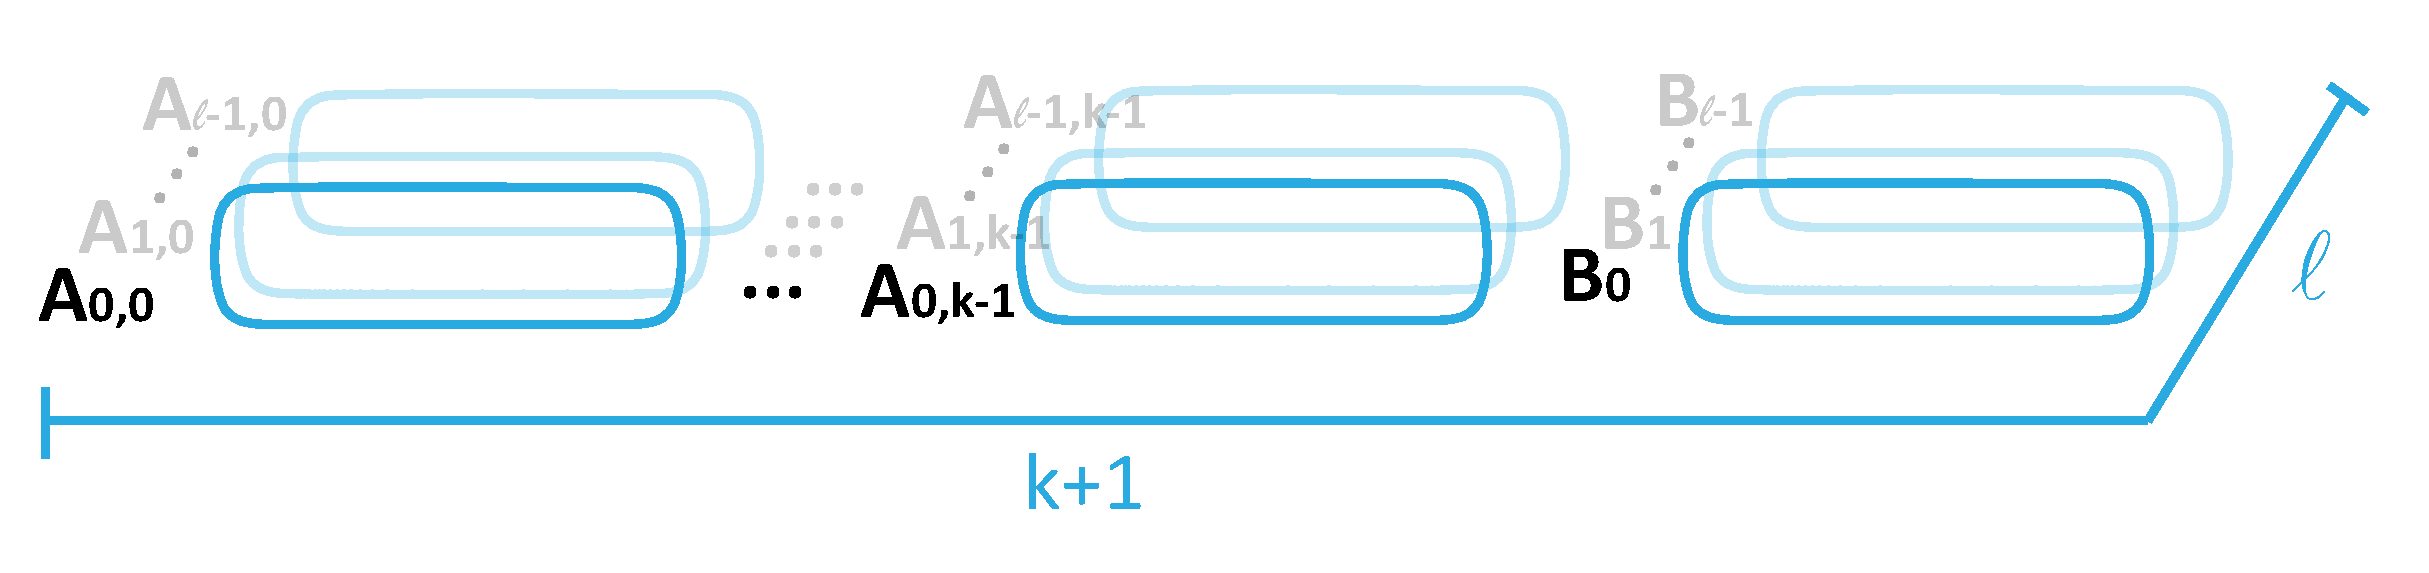
\includegraphics[width=1.0\linewidth]{figures/TFHE-fig2.pdf}
  \caption{An illustration of a GLev ciphertext }
  \label{fig:glev}
\end{figure}


\begin{comment}
\subsubsection{Discussion}

Suppose that the level $l$ of GLev is sufficient enough to fully decompose $M$ (\autoref{sec:decomp}), that is: 

$M = \dfrac{q}{\beta^1}M + \dfrac{q}{\beta^2}M + \gap{$\cdots$} + \dfrac{q}{\beta^l}M $

$ $

\noindent Then, summing all elements of $\textsf{GLev}_{S, \sigma}^{\beta, l}(M)$ is equal to $\textsf{GLev}_{S, \sigma}(M)$, because:

$= \textsf{GLWE}_{S, \sigma}\left(\dfrac{q}{\beta^1}M\right) + \textsf{GLWE}_{S, \sigma}\left(\dfrac{q}{\beta^2}M\right) + \gap{$\cdots$} + \textsf{GLWE}_{S, \sigma}\left(\dfrac{q}{\beta^l}M\right)$ 

$= \textsf{GLWE}_{S, \sigma}\left(\dfrac{q}{\beta^1}M + \dfrac{q}{\beta^2}M + \gap{$\cdots$} + \dfrac{q}{\beta^l}M \right) $ \textcolor{red}{\# We will prove this step later  in \autoref{sec:glwe-add-cipher}}

$= \textsf{GLWE}_{S, \sigma}(M)$

$ $

\noindent We will later leverage this property to implement TFHE's homomorphic multiplication (\autoref{subsec:tfhe-mult-cipher}).

\end{comment}

\subsection{Decryption}

It is sufficient to decrypt the GLev ciphertext's any $i$-th GLWE ciphertext by using the secret $S$, with the scaling factor $\Delta_i = \dfrac{q}{\beta^i}$.


\subsection{Lev and RLev}

Lev is GLev with $n=1$. RLev is GLev with $k=1$.


%\begin{figure}[h!]
%    \centering
%  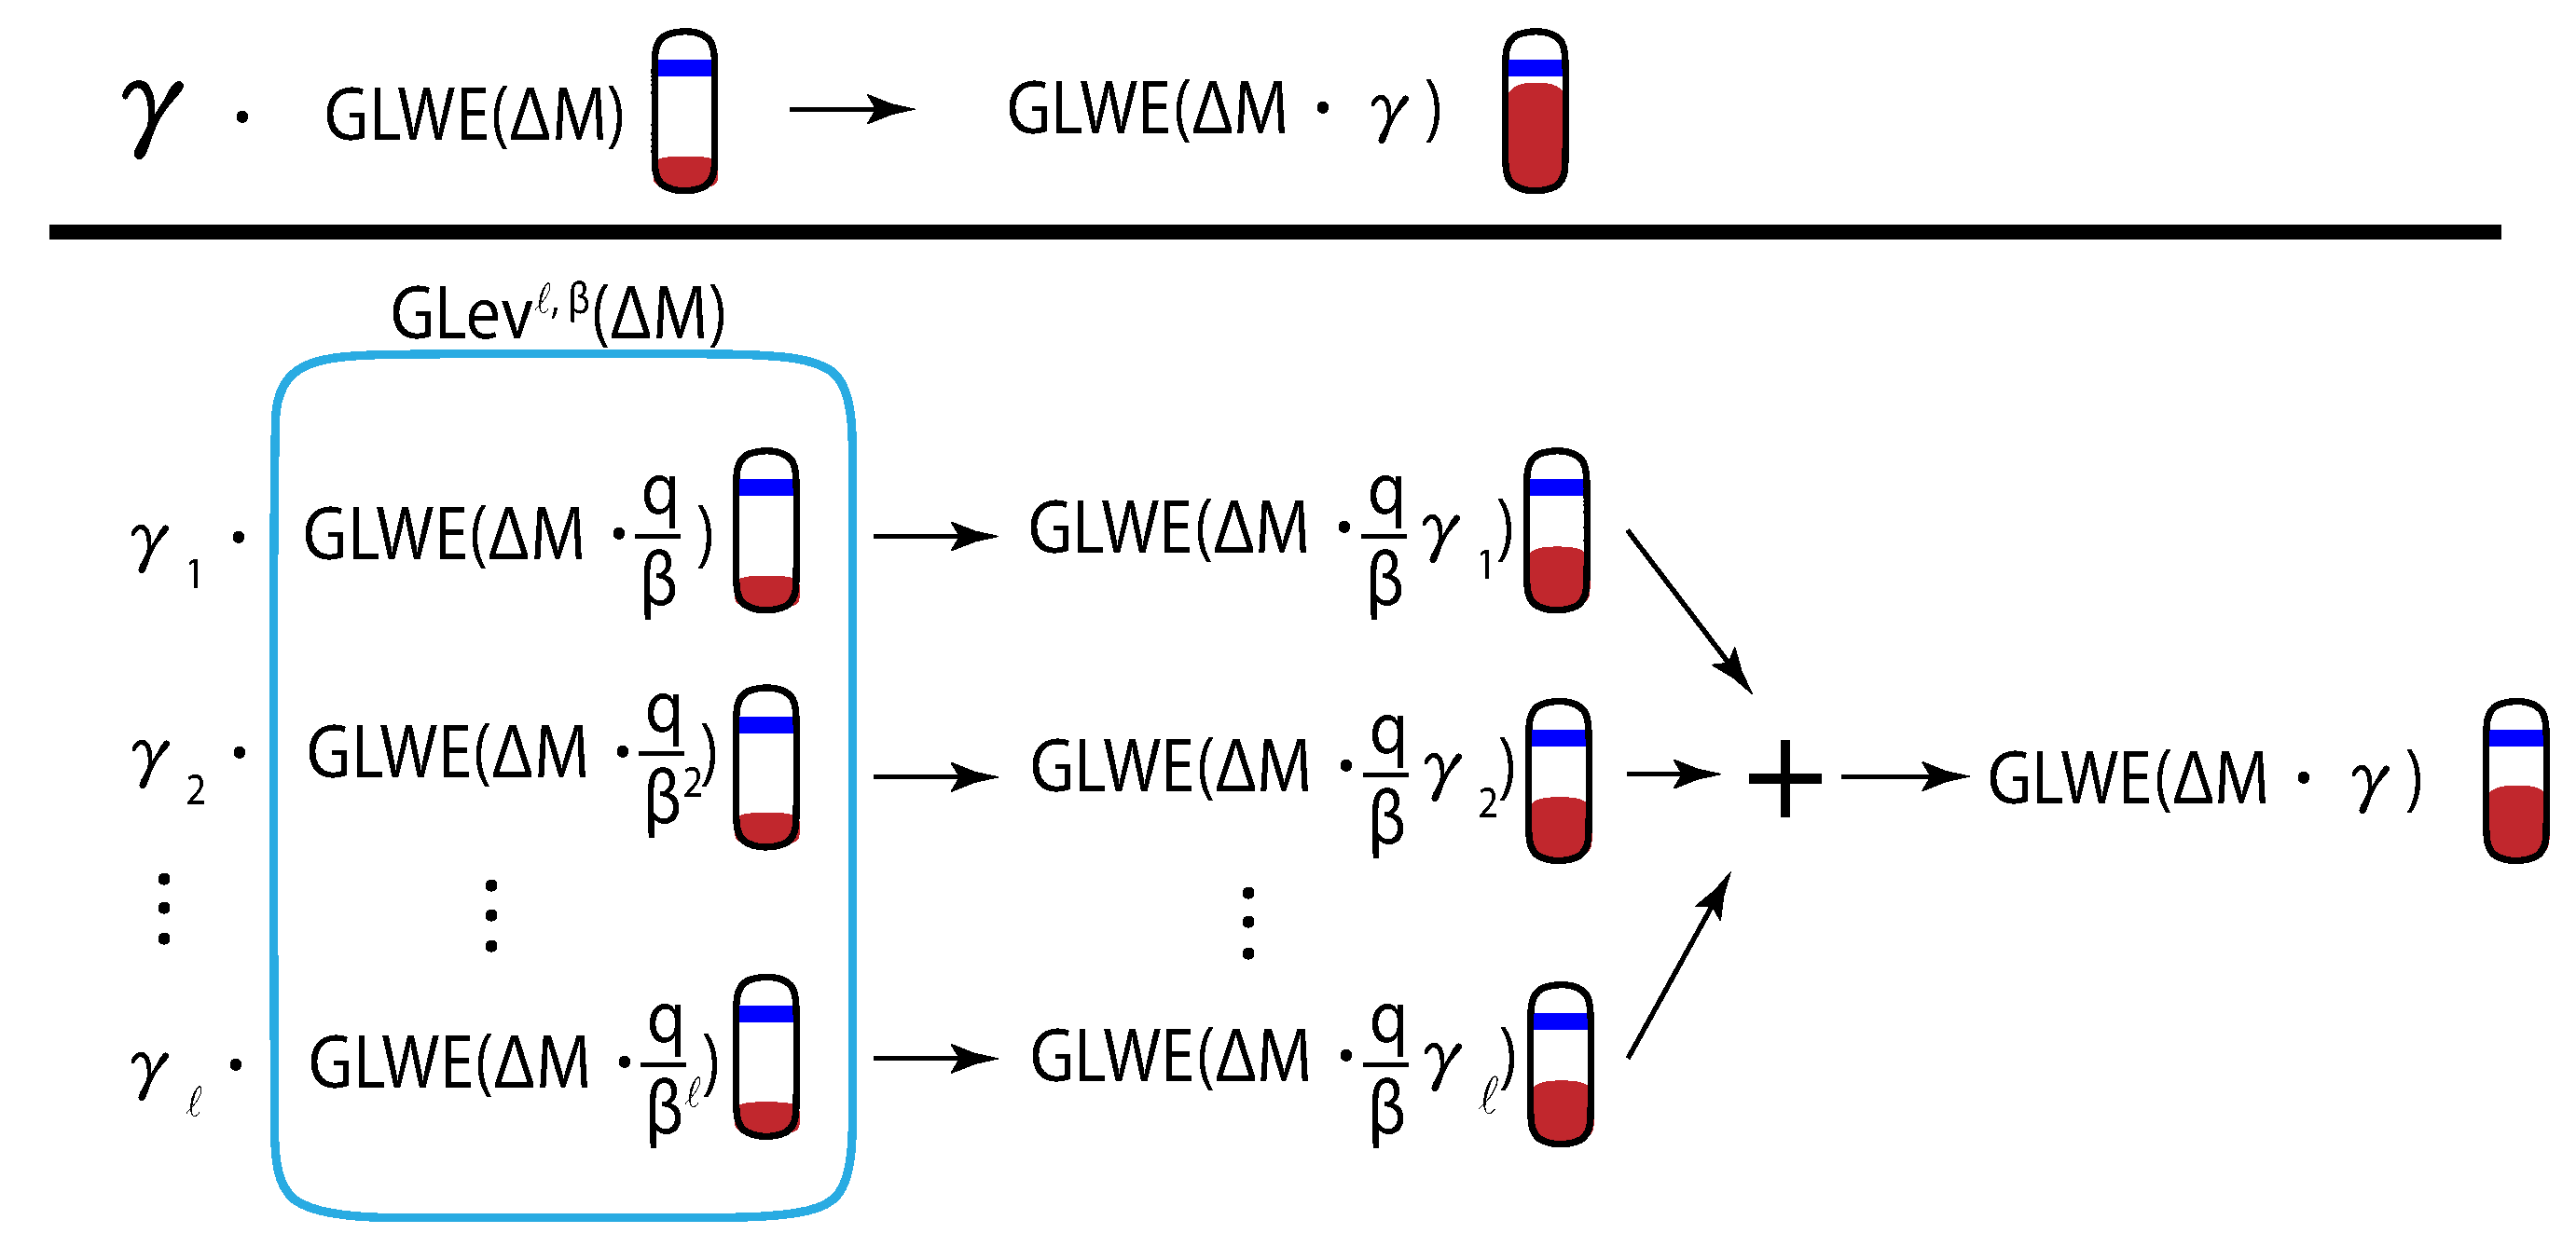
\includegraphics[width=1\linewidth]{figures/decomp2.png}
%  \caption{An illustration of a GLev ciphertext.}
%  \label{fig:decomp2}
%\end{figure}
